\documentclass{beamer}

\title{Short Introduction to Tor}
\subtitle{https://cryptoparty.dk}
\author{Ronni Elken Lindsgaard \\ \textless rel@zx.dk\textgreater}
\date{2015-01-24}

\usetheme{Malmoe}

\begin{document}

\begin{frame}
  \maketitle
\end{frame}

\begin{frame}
	\tableofcontents
\end{frame}

\section{What is Tor}
\begin{frame}
	\begin{block}{Trivia}
		\footnote{\url{https://en.wikipedia.org/wiki/Tor_\%28anonymity_network\%29}}
		\begin{itemize}
			\item Tor is acronym for The Onion Router
			\item Is infamously known in the media as ``The Dark Web''
			\item mid 1990s Onion Routing was developed
			\item In 2002 the first alpha version of Tor was released
			\item In 2004 Tor was released as free and open source
			\item In 2006 The Tor Project was founded
		\end{itemize}
	\end{block}

	% \begin{block}{Tor Family}
	% 	\begin{itemize}
	% 		\item Tails (OS on a stick)
	% 		\item Orbot (Android browser)
	% 		\item Stem (Dev library)
	% 		\item \ldots
	% 	\end{itemize}
	% \end{block}
\end{frame}
\begin{frame}{Users of Tor}
	\begin{itemize}
		\item Journalists
		\item IT Professionals
		\item People that
			\begin{itemize}
				\item Want to protect their privacy
				\item Hide from targeted marketing
				\item Want to access censored websites
				\item Blog/tweet without being traced
				\item ...
			\end{itemize}
		\item Human rights activists (HRW, EFF, \ldots)
		\item Military
		\item Intelligence agencies
		\item \ldots
	\end{itemize}
	\footnotetext{\url{https://www.torproject.org/about/torusers.html.en}}
\end{frame}

\section{Tor in a Nutshell}
	\begin{frame}{Terminology}
		\begin{block}{Tor}
			\begin{itemize}
				\item Bridge Node
				\item Relay
				\item Exit Node
			\end{itemize}
		\end{block}

		\begin{block}{Crypto}
			\begin{itemize}
				\item Alice
				\item Bob
			\end{itemize}
		\end{block}
	\end{frame}
	\begin{frame}{Directory listing}
		\begin{center}
			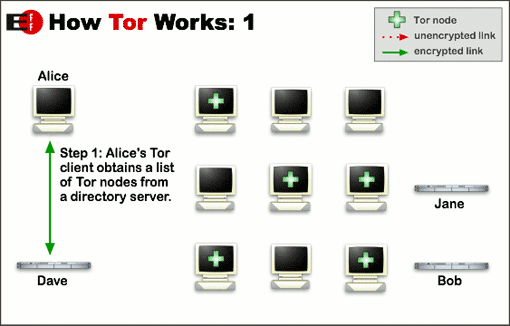
\includegraphics[width=0.7\textwidth]{htw1.png}
		\end{center}
		\footnotetext{Source: \url{https://www.torproject.org/about/overview.html.en}}
	\end{frame}
	\begin{frame}{Onion Routing}
		\begin{center}
			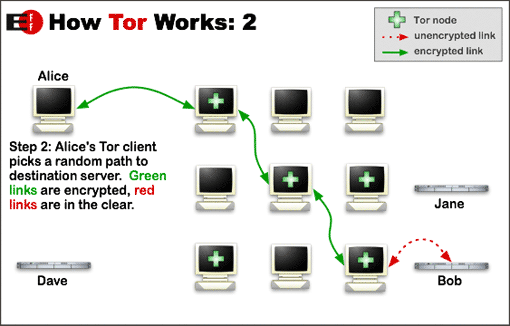
\includegraphics[width=0.7\textwidth]{htw2.png}
		\end{center}
	\end{frame}
	\begin{frame}{Not Entirely Unlike Ogres}
		\begin{center}
			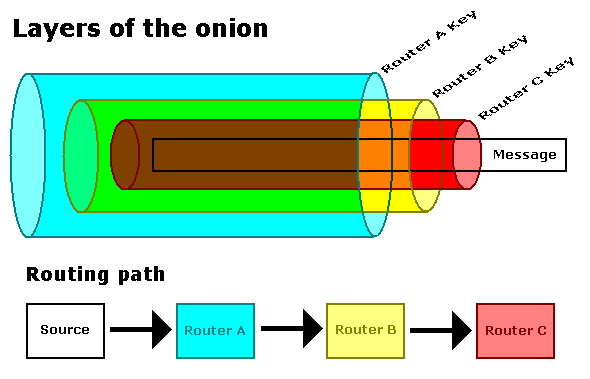
\includegraphics[width=0.7\textwidth]{layers.png}
			\footnotetext{\url{https://upload.wikimedia.org/wikipedia/commons/7/7d/Onion_diagram.png}}
		\end{center}
	\end{frame}
	\begin{frame}{Anonymity}
		\begin{center}
			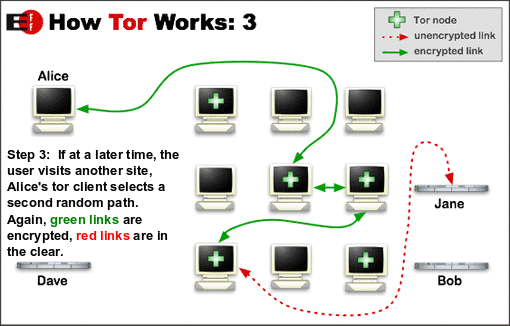
\includegraphics[width=0.7\textwidth]{htw3.png}
		\end{center}
	\end{frame}

\section{Dos and Don'ts}
\begin{frame}
	\begin{block}{Do}
		\begin{itemize}
			\item Use it when you need anonymity
			\item Use it to help others obtain anonymity by
				\begin{itemize}
					\item Setting up a Tor node
					\item Use Tor responsibly
				\end{itemize}
			\item Learn more
		\end{itemize}
	\end{block}

	\begin{block}{Don't}
		\begin{itemize}
			\item Download binaries
			\item Use it for illegal purposes
			\item Torrent
			\item Trust anything blindly
		\end{itemize}
	\end{block}
\end{frame}

\begin{frame}{Important notice!}
	\begin{center}
		\huge{Being anonymous on the internet does not allow you to hurt people or to be an asshole!}
	\end{center}
\end{frame}

\section{Hidden Services}
	\begin{frame}{Hidden Services}
		\begin{itemize}
			\item Anonymous sender \textit{and} receiver
		\end{itemize}
		\begin{center}
			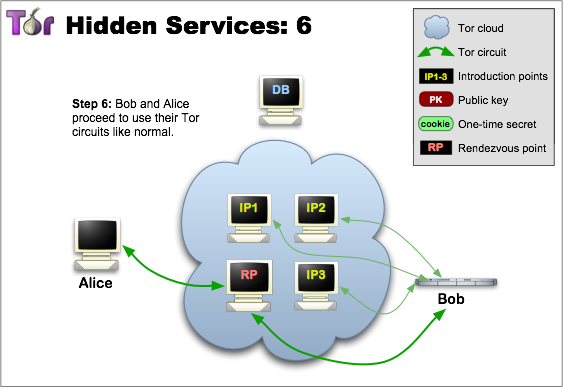
\includegraphics[width=0.7\textwidth]{THS-6.png}
		\end{center}
		\footnotetext{\url{https://www.torproject.org/docs/hidden-services.html.en}}
	\end{frame}

\section{Where to go from here}
	\begin{frame}{Resources}
		\begin{description}
			\item[WWW] \url{https://torproject.org}
			\item[IRC] \#tor on irc.oftc.net
			\item[Mail] \url{https://lists.torproject.org/cgi-bin/mailman/listinfo/tor-talk/}
			\item[Slides] \url{https://github.com/rlindsgaard/presentations/2015-01-24-short-introduction-to-tor/}
		\end{description}

		\begin{center}
			\#cryptopartycph on irc.freenode.net
		\end{center}
	\end{frame}
\end{document}